
\section{Bars}
\index{secrets!bars}

Tinn-R has three bars. The top task bar is related to the application and editor,
the second task bar is focused on \RR{}, and the bottom bar displays the program status.

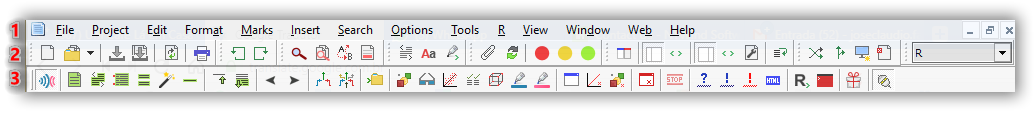
\includegraphics[scale=0.50]{./res/parts_02.png}
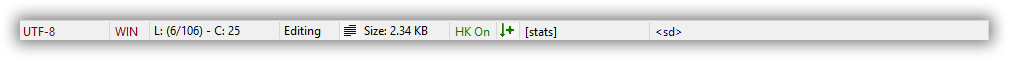
\includegraphics[scale=0.50]{./res/status_bar.png}

The top task bar (2) can have its location modified by draggin and dropping with your mouse.
Right click anywhere on top task bar (2) to see the pop-up menu where you can choose which box
of the bar you would like to show or hide. Every box of that bar has a vertical line at its left side.
Right click at that location and you can move the bar up and down.

The \RR{} task bar (3) can be moved wherever you wish. Right click the vertical line at the left side of the
bar and move it across either the editor or \texttt{Rterm}. Right click anywhere within the \RR{} task bar and choose between
\texttt{Send to \RR{}} and \texttt{Control \RR{}} to have them displayed or hidden.

The status bar at the bottom of the editor window, shows the current line you are working on,
the total number of lines, and the current column at the first box.
It also shows the modes which can be either \texttt{normal or read only}.
You are not allowed to make any changes in the \texttt{read only} mode.
There is also information about selection mode. It allows you to change the way you select parts of the current working file.
See \textit{\href{\#secrets\_after\_installation}{After installation}}.
